% Simple level diagram of Cr-51.
% Zhu Baoji, 2018

\documentclass[10pt]{article}
\usepackage{tikz}
\usetikzlibrary{arrows}
\usetikzlibrary{calc}

\begin{document}

% Place the TikZ picture in a figure environment.
\begin{figure}
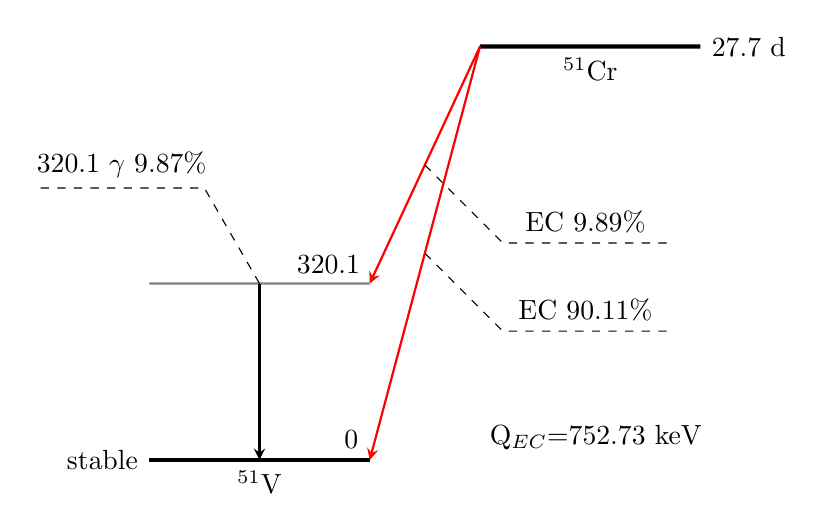
\begin{tikzpicture}[
      scale=0.7,
      level_stable/.style={ultra thick},
      level/.style={gray,thick},
      trans/.style={thick,->,>=stealth},
    ]
    \coordinate (L1_a) at (2,7.5);
    \coordinate (L1_b) at ([shift={+(4,0)}] L1_a);
    \coordinate (L2_a) at (-4,3.2);
    \coordinate (L2_b) at ([shift={+(4,0)}] L2_a);
    \coordinate (L3_a) at (-4,0);
    \coordinate (L3_b) at ([shift={+(4,0)}] L3_a);
    % Draw the energy levels.
    \draw[level] (L2_a) -- (L2_b);
    \node[above left] at (L2_b) {320.1};
    \draw[level_stable] (L1_a) -- (L1_b) node[right] {27.7 d} node[midway,below]{$^{51}$Cr};

    \draw[level_stable] (L3_b) node[above left]{0} -- (L3_a) node[left] {stable} 
        node[midway,below]{$^{51}$V};
    % Draw the transitions.
    \draw[trans,red] (L1_a) -- (L2_b);
    \coordinate (T1) at ($ (L1_a)!.5!(L2_b) $);
    \coordinate (T1_2) at ([shift={+(-45:2)}] T1);
    \coordinate (T1_3) at ([shift={+(3,0)}] T1_2);
    \draw[dashed] (T1) -- (T1_2) -- (T1_3) node[midway,above]{EC 9.89\%};

    \draw[trans,red] (L1_a) -- (L3_b);
    \coordinate (T2) at ($ (L1_a)!.5!(L3_b) $);
    \coordinate (T2_2) at ([shift={+(-45:2)}] T2);
    \coordinate (T2_3) at ([shift={+(3,0)}] T2_2);
    \draw[dashed] (T2) -- (T2_2) -- (T2_3) node[midway,above]{EC 90.11\%}; 

    \coordinate (L2_c) at ($ (L2_a)!.5!(L2_b) $);
    \coordinate (L3_c) at ($ (L3_a)!.5!(L3_b) $);
    \draw[trans](L2_c) -- (L3_c);
    \coordinate (T3_1) at ([shift={+(120:2)}] L2_c);
    \coordinate (T3_2) at ([shift={+(-3,0)}] T3_1);
    \draw[dashed] (L2_c) -- (T3_1) -- (T3_2) node[midway,above]{320.1  $\gamma$ 9.87\%};
    
    \coordinate (Q1) at ([shift={+(2,0)}] L3_b);
    \node[above right] at (Q1) {Q$_{EC}$=752.73 keV}; 
\end{tikzpicture}
\end{figure}

\end{document}
